\chapter{{Overview of text elements in film – Translation and graphical impact}}\label{overview}


According to multiple award-winning film editor Walter Murch, emotion “is the thing that you should try to preserve at all costs” (\citealt{murch2001}:~18) when editing film.\footnote{Parts of this chapter have been published previously in the article “Should she really be covered by her own subtitle? – Text elements in film and their \isi{graphical translation}”, Translation Spaces 5:~2 (2016), 244--270.} Similar to film editors, translators should always understand a scene’s emotion and atmosphere and try their best to recreate them. They should be aware that even the decision whether or not to translate a text element, and in which way, can be considered as much an act of interpretation as the content translation itself. Ideally, the audience should never wonder about a missing or unnecessary translation – or why that subtitle just moved to the top and now covers the speaker. While being historically a \isi{dubbing country}, more and more German viewers prefer the original version of English film productions, and DVDs and Blu-rays released in Germany usually include subtitles nowadays. However, subtitling does not only create timing, space and content challenges but also graphical challenges related to the collision of additional text elements (subtitles) with pre-existing text elements (e.g. captions); it changes the information flow and reception of the image (cf. \citealt{rayner2001}; \citealt{Caffrey2009}; \citealt{romero-fresco2013}) and possibly influences the audience’s \isi{overall aesthetic experience}. So far, little thought has been given to the influence that translations of text elements in film have on \isi{image composition} and reception and they are rarely considered an interwoven unity.

Therefore, this chapter provides an overview of text elements in general, strategies used in their \isi{graphical translation} from English into German, and the concept of \isi{typographic identity} as a basis for the discussion of creative alternatives and developments.

\section{Representative film corpus}\label{sec:2.1}

The examples discussed in this chapter were taken from a film corpus that was created solely for this purpose (see Appendix A). The corpus is based on the following four top 100 lists of the most popular films published between and including 2000 and 2009:

\begin{itemize}
\item Top-grossing feature films in the USA\footnote{Cf. \url{http://www.imdb.com/search/title/?release\_date=2000,2009\&sort=boxoffice\_gross\_us\& title\_type= feature} [2016--07--27].}
\item Top-grossing feature films in Germany\footnote{Cf. \url{http://www.insidekino.de/DJahr/D2000--2009.htm} [2016--07--27].}
\item Top-rated feature films on METAcritic (both critics and users)\footnote{Cf. \url{http://www.metacritic.com/feature/the-best-movies-of-the-decade} [2016--07--27].}
\item Most popular feature films on IMDb\footnote{Cf. \url{http://www.imdb.com/search/title/?release\_date=2000,2009\&title\_type=feature} [2016--07--27].}
\end{itemize}

Each of the films in these top 100 lists was assigned a score between 1 and 100 depending on its rank in the list (the highest-ranked film receiving a score of 100 and so on). Based on these scores, a mean score was calculated for each film mentioned in the lists. The 100 English language films with the overall highest scores were included in the final corpus. Therefore, it can be assumed that these are the 100 English language films with the strongest impact in Germany in these ten years. The corpus constitutes a representative sample of the English film industry in the 2000s and, as such, enables a detailed analysis of recent strategies in regard to design and translation of text elements, as well as the film-specific identity that can be created through the well thought-out use of \isi{typography}. So far, 52 of the 100 films in the corpus have been thoroughly analysed and annotated (see Appendix A for details). These films constitute the basis for the statistics used throughout this chapter. The selection of films is a convenience sample based on availability. Other films from the corpus are used in order to illustrate specific and rare occurrences that did not occur in the analysed films. Films that are not part of the corpus but are required to illustrate cases that did not occur in the sample are marked accordingly.

The text elements were analysed using the English audio and image track as well as the German subtitles. As DVD or Blu-ray Disc (BD) descriptions do not specifically state which image tracks are included, and the contents of the data carriers can vary a lot, this feature was not analysed for all films in the corpus. This point is, however, explained in more detail in the section on technical considerations and some examples are provided. Further variations can occur between cinematic versions, TV versions, and commercial versions and were not recorded in this corpus. The analysis includes films from DVD, BD, and the two online streaming services \textit{Amazon Prime} and \textit{Netflix}.\footnote{Currently, these are the only major streaming providers in Germany that offer subtitles (cf.\,\url{http://www.netzwelt.de/video-streaming/kaufberatung-video-streaming-dienste-test-netflix-amazon-prime-maxdome-co-vergleich.html} [in German; 2016--06--03]).} The format and version (regular, special edition, extended edition) of the respective films were based on convenience and not marked in the corpus.

\section{Technical considerations}\label{sec:2.2}

Several technical constraints should be taken into consideration due to not only the wide range of formats films can be watched in but also the variations within these formats. As mentioned before, the database includes films analysed on DVD, BD, \textit{Amazon Prime}, and \textit{Netflix}. These data carriers and providers mostly vary in terms of average file size, image resolution, and applied strategies concerning the use of image tracks. DVDs can either be single or double layer and can store 4.7~GB or 8.7~GB, corresponding to approximately 2 or 4 hours of standard definition information (SD, 480--540p). BD offers 25~GB and 50~GB of capacity, equating approximately 2 or 3~hours respectively of high-quality information (720/1080p) “with additional room for 2~hours [or 9~hours, resp.] of bonus material in SD quality” (\citealt{Blu-ray_disc_association2015}). The online streaming services provide image resolutions of up to 4k/UHD (2160p) with corresponding file sizes. The difference in storage size between DVD and BD can be traced to the two different lasers that are used to read the information: While DVD is read by red lasers (650nm), BD uses blue lasers (405nm) that, due to their shorter wave length and therefore smaller size of focused laser spot, allow for almost five times the number of grooves and therefore a much higher storage capacity.

The data stored on these devices and platforms that are relevant for this article are the image tracks, audio tracks, and subtitle tracks. Depending on the publisher, English films in Germany can be available with the original English (unaltered) image track, the German image track that features substitutions of text elements, or both. Image tracks in one language version but with various different cuts (such as the official cinema cut versus the director’s cut or an extended cut) are also possible. Furthermore, the option to have one major image track that only offers versions in which there are actually (translated) text elements in a scene also exists. This, as well as the various cut versions, is achieved by “\isi{seamless branching}” (\citealt{tfdvd_research_labs2005}) or the ‘misuse’ of the multi-angles option. The multi-angle option was originally intended to offer several perspectives of specific scenes. Today, while it is still used in some genres such as recorded live concerts, it is mostly used for internationalisation purposes – this version will, depending on the audio track and whether a scene has a translated version in that language, replace the source language version. Similar to this use of multi-angle videos,
\begin{quote}
the technique of \isi{seamless branching} uses a special type of interleaving […], where multiple versions of the video are woven together into “angle blocks”, and then the bits which “aren’t playing” are skipped over during decoding/playback. (\citealt{tfdvd_research_labs2005})
\end{quote}
While the information on use or existence of these multiple language versions of the image track are not included in the technical (or any) DVD and BD description, German \textit{Netflix} client support states that they only offer the original image track provided by the studios.\footnote{As stated during the communication with the German \textit{Netflix} client support [2016--06--01].} \textit{Amazon Prime}, on the other hand, states that they offer one or both image tracks depending on the provider and link it to the corresponding audio track.\footnote{As stated during the communication with the German \textit{Amazon Prime} client support [2016--06--03].} Judging from personal experience, this feature is mostly used if the main target group is children – see for example \textit{The Incredibles} (USA 2004) – or if the use of specific text elements is crucial to the film’s atmosphere or plot, e.g. all films in the \textit{Star Wars} (USA 1977-) franchise or \textit{Avatar} (USA/UK 2009).

The number and quality of audio tracks on both DVD and BD depend on the remaining space with a limit of eight audio tracks on DVD and no limit on BD.\footnote{Limits of data rates and balance of features on BD are discussed in detail in various BD forums, e.g. \url{http://www.bluray-disc.de/forum/dokus-und-musik-auf-blu-ray/76647-musik-bd-welche-audioformate-und-was-geht.html} [in German; 2016--06--03].} These audio tracks are used for different audio formats and different languages. Audio tracks that provide an alternative language are usually linked to the corresponding image track, if available. Even though there is no audio track limit for the streaming providers, \textit{Amazon Prime} usually only provides the source language (if at all) and the German dubbed version, while \textit{Netflix} seems to usually offer the English source version, the German dubbed version if available, and sometimes dubbed versions in other languages, such as French. This also seems to depend on the issuing studios as well as licensing costs.

Finally, there are usually multiple subtitle tracks included in DVD and BD publications. \textit{Amazon Prime} offers a growing number of films with English and German subtitles and \textit{Netflix} usually offers at least English and German subtitles as well as a wide range of other languages. Subtitle tracks in the corpus included English subtitles, English subtitles for the \isi{deaf} and hard-of-hearing (SDH), German subtitles, German SDH, commentaries, other language subtitles, and subtitles for an \isi{additional language} in the film.\footnote{For example, the BD of \textit{The Lord of the Rings – The Two Towers} (USA/NZ 2002) includes an English subtitle track that only translates the Elvish dialogues as well as a German subtitle track that provides the corresponding German translations. Ideally, these are linked to the corresponding audio tracks and displayed by default. If not, they are easily missed as one of many subtitle tracks, and the information of these dialogues is lost. On BD, individual subtitles can be marked as ‘forced’ subtitles and will be shown regardless of player settings.} The \isi{layout} of the subtitles depends largely on the production company. \textit{Amazon Prime} and \textit{Netflix} offer a wide range of individual \isi{subtitle appearance} settings (see \figref{fig:FIG1}). While \textit{Amazon Prime} allows users to set the size and choose one of four overall \isi{layout} pre-sets, \textit{Netflix} offers seven fonts, five different shadow settings, and various colours for either a background or box behind the subtitle, including semi-transparency.

\begin{figure}
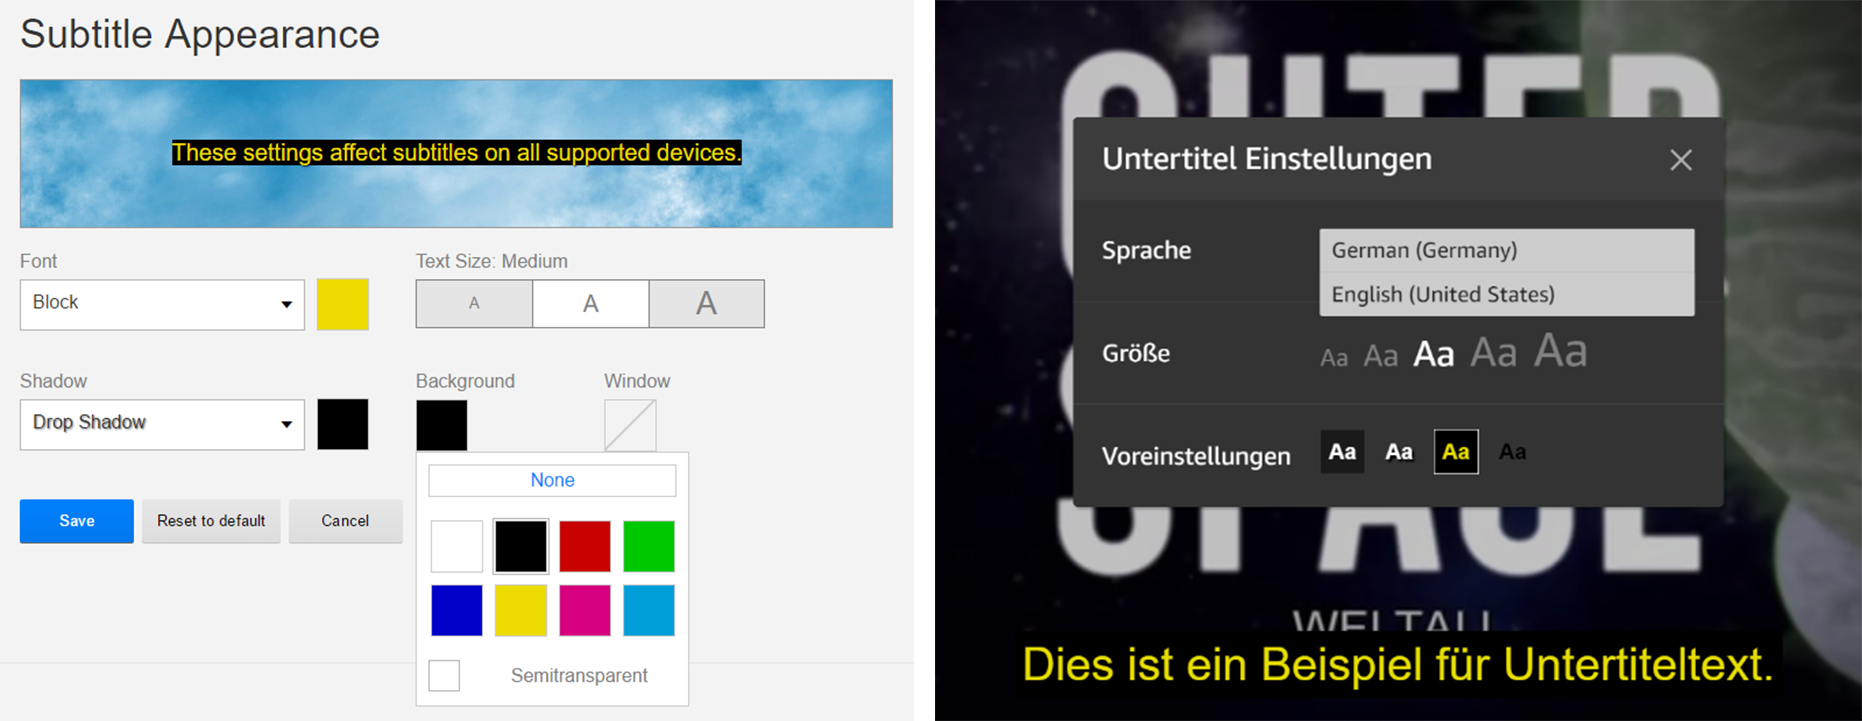
\includegraphics[width=\textwidth]{figures/FIG1.png}
\caption{Configuration of subtitle appearance on \textit{Netflix} (left) and \textit{Amazon Prime}  (right).}
\label{fig:FIG1}
\end{figure}

On DVD and BD, this is very different. Subtitles are saved as image files on both DVD and BD\footnote{Cf. \url{http://en.flossmanuals.net/avidemux/ch019\_extract-dvd-subtitles/} [2017--06--06] for DVD and \url{http://forum.videohelp.com/threads/313620-How-to-extract-subtitles-from-a-Blu-ray-and-convert-to-srt-or-sub-idx} for BD [2016--06--06].} and their overall \isi{layout} cannot be adjusted by the viewer or playback device. While most studios stick to the traditional white subtitles with black border or shadow in the bottom-centre area, some recent BDs offer individually placed English SDH, e.g. \textit{Gone Girl} (USA 2014) and \textit{Ex Machina} (UK 2015; see \sectref{sec:4.1}). This was not observed on any other medium.

Due to this wide range of formats, layouts and combinations thereof, the decision was made to limit this first analysis to the provided image track – either the original English image track or the German image track – and German subtitles. As \isi{subtitle layout} differs significantly depending on individual settings (streaming) or playback devices (DVD and BD), only the \isi{layout} of the original text elements and their translations will be taken into account. It often creates its own, individual character, or even, identity.

\section{Typographic film identity}\label{sec:2.3}

Even before spoken language, written text was part of filmmaking – from the first silent films on, text appeared “in the form of title cards for opening, closing and intertitles, as subtitles, abstract character code or single character, as independent theme, image or calligraphy or ornament” (\citealt{Ehrenhauser2007}:~3, author‘s translation). Genre-independent, various kinds of written text are used in illustrative and explanatory ways in the moving image.

These text elements and their design often create a strong identity that can make a film more distinctive and add further \isi{recognition value}. For example, a well thought-out and distinctive film \isi{title design} can allow for easy recognition, even without the original text. During the \isi{translation process}, however, films are edited both in additive and substituting ways – be it the addition of subtitles or the substitution of the audio channel. Both forms of audiovisual translation include, depending on target group and applied guidelines, the translation and recreation of relevant text elements. This translation of both spoken and written language can result in a noticeable interference with the \isi{typographic film identity} as written translations are added or replace existing text elements.

But how is this \isi{typographic film identity} created and what makes viewers remember certain aspects of a film such as the \isi{title design} or an opening sequence? It is the design. And it is not only the more obvious aspects such as the main colours of the images (think of the distinctive blue-green of \textit{Avatar}) or especially \isi{aesthetic} shots. The film’s design also includes all the \isi{typographic} elements, their typefaces, \isi{placement}, effects, and colours. The overall use of text elements can support or establish a specific tone or atmosphere – just as it was intended and implemented in \textit{John Wick} (USA 2014): When asked why they chose integrated titles, the two filmmakers Chad Stahelski and David Leitch replied that it had to do with tone: “Most people use subtitles to get across information or do what they are there for, translation. We needed hints with tone” \citep{Graham2014}. Many typefaces evoke specific associations or emotions due to their established use. The same holds true for effects and \isi{placement} strategies. Atmosphere and emotions can create continuity and strengthen the \isi{recognition value} – similar to branding strategies and \isi{corporate design}. This, however, should not be confused with marketing, even though they are strongly related: “Branding is not actively selling but representing: ‘This is what I am.’” \citep{Heaton2011}. Corporate design, as a part of the complexity that is corporate identity, is the design of “all visual forms of expression of a company” (\citealt{Weinberger2010}:~55) that provides the “most significant distinction” (\citeyear{Weinberger2010}:~55) and “strongest \isi{recognition value}” (\citeyear{Weinberger2010}:~55). Weinberger defines a number of essential elements of \isi{corporate design} (\citeyear{Weinberger2010}:~55): Logo, colour, shapes, \isi{typography}, \isi{communication design} (all printed and digital material), industrial design (packaging), images (moving and still images), architecture, clothing, and CD manual. Apart from architecture, most of these elements can be found in film production. In regard to \isi{typographic film identity}, the \isi{film title} is often used as a logo (see the \textit{Harry Potter} [UK/USA 2001--2011] or \textit{The Lord of the Rings} [NZ/USA 2001--2003] franchises), and colour, shapes, and \isi{typography} can be found in the text elements of a film. This kind of branding or \isi{corporate design} often even affects the studio logos in recent films, adjusting to the film’s overall design\footnote{Other aspects of this overall design are a film’s motion design, e.g. opening titles and elements added in the post-production, props (cf. Annie Atkins, designer for the \textit{Grand Budapest Hotel} (USA/DE/FR 2014), \url{http://create.adobe.com/2015/12/2/the\_secret\_world\_of\_annie\_atkins\_graphic\_designer\_for\_films.html} [2016--06--03]), and elements created by video designers in the post-production, e.g. visualised text messages.} – as seen for example in the \textit{The Matrix}  films (USA 1999--2003), where the Warner Brothers logo is tinted green and looks more “computerish”\footnote{Cf. \url{http://www.closinglogos.com/page/Logo+Variations+-+Warner+Bros.+Pictures} [2016--06--03] for examples on Warner Bros. and \url{http://www.closinglogos.com/page/Logo+Variations+-+20th+Century+Fox+Film+Corporation} for Twentieth Century Fox [2016--06--03].} (\citealt{quitsch2010}:~48ff.).

\largerpage 
While an overall film design includes most of the aspects that can be found in a \isi{corporate design}, the text elements form a distinctive group – creating a \isi{typographic film identity}. Led by the \isi{film title}, the ‘logo’, text elements in the film usually follow a specific design, captions are presented in one \isi{typeface} and colour throughout the film, and even displays might look similar or are filmed in a similar way. The same is true for inserts, opening and closing credits, and \isi{narrative text} elements (for an example, see \figref{fig:FIG2}).

\clearpage 
\begin{figure}[t]
\includegraphics[width=\textwidth]{figures/FIG2.png}
\caption{Overall typographic identity in \textit{Seven Pounds} (USA 2008)}
\label{fig:FIG2}
\end{figure}

  
In the course of translation, however, text elements are often subtitled or replaced. As explained in the technical considerations section, the design of subtitles usually depends on either the studio or the streaming platform. On the one hand, subtitles, as a major \isi{typographic} influence on the film, should ideally become a part of its \isi{typographic identity} or create as little interference as possible – but this is usually not the case. If taken into account, however, subtitles could probably reinforce the \isi{typographic identity} which supports the film’s atmosphere. This was done, to some extent, in \textit{Avatar}.


As can be seen in \figref{fig:FIG3}, the burnt-in subtitles for the additional alien language were not the only aspect that was adapted to the film’s dominant colours – creating the best possible visibility by contrasting the blue and green image with yellow subtitles – but the optional subtitles also follow the basic \isi{typographic identity} of the film. Similar approaches were used in the \textit{The Lord of the Rings} franchise, creating film-specific fonts and applying elaborate \isi{serif} typefaces for the forced Elvish language subtitles.\footnote{For an overview of the typefaces created for the franchise, see for example \url{http://www.theonering.net/torwp/2014/06/26/90498-the-lord-of-the-fonts-a-guide-to-fonts-in-the-hobbit-and-the-lord-of-the-rings/2/} [2016--06--06].}

\begin{figure}[t]
\includegraphics[width=\textwidth]{figures/FIG3.png}
\caption{Forced subtitles (left) and optional subtitles (right) in \textit{Avatar} (00:42:07, 00:12:25)}
\label{fig:FIG3}
\end{figure}

On the other hand, typefaces that are too specific and associated with other genres might not be adequate for the atmosphere of some film and irritate the audience – see for example the futuristic subtitles in the WWII historical comedy \textit{Train of Life} (FR/BE/NL/ISR/ROU 1998) in \figref{fig:FIG4} (on the left). Additionally, interference might occur due to the dominance of a subtitle in a scene with otherwise muted colours and text elements (see \figref{fig:FIG4} on the right).

\begin{figure}[t]
\includegraphics[width=\textwidth]{figures/FIG4.png}
\caption{Typographic and thematic interference in \textit{Train of Life} (00:12:23) and in \textit{In Bruges} (UK/USA~2008, 00:01:31)}
\label{fig:FIG4}
\end{figure}

\figref{fig:FIG5} shows the BBC television series \textit{Sherlock} (UK/USA 2010-) and its translation into German. While \textit{Sherlock} is a great example of the intelligent use and design of text inserts, the German version is an example of how to sometimes overlook \isi{typographic} details. While it might be understandable that not the exact same \isi{typeface} was used, the change from \isi{sans-serif} to a \isi{serif} \isi{typeface} was unnecessary – and can possibly lead to a minor change of atmosphere in the corresponding scenes. While the \isi{sans-serif} \isi{typeface} in the original suggests a modern context in the age of smartphones and texting, the \isi{serif} \isi{typeface} in the German translation is associated with a rather different area of application: Serif typefaces require a higher resolution to be presented clearly and are therefore hardly used on phone screens. They are traditionally associated with printed type faces and books – not the digital world (see \figref{fig:FIG5}).

\begin{figure}
\includegraphics[width=\textwidth]{figures/FIG5.png}
\caption{Original \textit{Sherlock} scene, close-up of the English text insert, and its translation (S01E01, 00:12:14)}
\label{fig:FIG5}
\end{figure}

\newpage 
Examples such as \textit{Sherlock} show that new expertise is required to deal with the various aspects of \isi{typographic film identity}. Only if existing \isi{layout} strategies and designs are understood and text elements and their value recognised, can they be recreated in a way that does not disturb the film’s atmosphere, tone, and overall identity.

\section{Text elements in film}\label{sec:2.4}
\largerpage
As previously explained, translation in film does not only involve spoken language but also written text elements in the source language. In the 52 analysed films, a total of 1170 text elements with the frequencies in \tabref{tab:TAB2} were observed.

\begin{table}
\begin{tabularx}{.8\textwidth}{Qrr}
\lsptoprule
 Element &  Count &  Percentage (\%)\\
 \midrule 
 Film title & 65 & 5.56\\
 Opening credits & 29 & 2.48\\
 Closing credits & 57 & 4.87\\
 Displays & 560 & 47.86\\
 Captions & 107 & 9.15\\
 Narrative texts & 10 & 0.85\\
 Inserts & - & -\\
 Subtitles & 342 & 29.23\\
 \midrule 
&  1170 &  100.00\\
\lspbottomrule
\end{tabularx}
\caption{Frequency of text elements in the 52 analysed films}
\label{tab:TAB2}
\end{table}

The following sections provide definitions and indicate the relevance of the individual text elements as well as challenges that arise due to their content and \isi{graphical translation}.

\subsection{Film title}\label{sec:2.4.1}

The \isi{film title} can be seen as one of the most relevant links between the original version and translated versions of a film – at least concerning marketing and presence. Ideally, it should be possible for the audience to make the connection between the original film and the German version. However, many German film titles such as “Welcome to the Jungle” (\textit{The Rundown}, USA 2003) or “Vergiss mein nicht!” (“Forget Me Not”, \textit{Eternal Sunshine of the Spotless Mind}, USA 2004)\footnote{See\,\mbox{\url{http://www.filmpilot.de/news/top-7-deutsche-filmtitel-die-uns-fuer-bloed-halten-109320}} for a list of various criticised or even faulty \isi{film title} translations from English into German [in German; 2016--05--11].} indicate that marketing decisions are not always based on what would be an obvious translation. As Bouchehri states, it is often agencies that create the original titles in the United States (\citealt{Bouchehri2008}:~30) and the distributors in Germany that choose a translation or new title (\citealt{Bouchehri2008}:~20). Therefore, the linguistic \isi{translation process} of film titles remains quite elusive.

The title, however, is not only relevant for marketing purposes but also for the \isi{overall image composition} and identity of a film. Of the 52~films analysed, all films included at least one scene with the \isi{film title} in it and 11 films showed the \isi{film title} more than once. If it is presented at the beginning of a film, it can create a specific atmosphere and shape the \isi{typographic identity} of the film – or subsequently strengthen it when presented after the film and before the closing credits (as in e.g. \textit{Avatar} and \textit{Hot Fuzz} [UK/FR/USA 2007]). Especially multi-part films and film series such as \textit{The Lord of the Rings} or \textit{Harry Potter} feature a clear and differentiated \isi{typographic identity} related to the \isi{film title} which creates \isi{recognition value} and strengthens the franchise. While the influence of the title translation on marketing is difficult to determine (\citealt{schreitmuller1994}:~72ff.), inconsistencies concerning the design or translation of the \isi{film title}\footnote{An example of inconsistency in translation would be the series of films \textit{Pirates of the Caribbean}. The first film, \textit{Pirates of the Caribbean} (USA~2003), was translated and marketed as “Fluch der Karibik” (Curse of the Caribbean). The second part \textit{Pirates of the Caribbean: Dead Man’s Chest} (USA~2006), obviously in an attempt to create at least some kind of continuity, was translated as “Pirates of the Caribbean – Fluch der Karibik 2” and only the third part follows the original title \textit{Pirates of the Caribbean: At World’s End} (USA~2007) with the translation “Pirates of the Caribbean – Am Ende der Welt”. The fourth part then followed the same strategy.} might lead to irritation. As film titles function as names (cf. \citealt{nord1993}:~87ff.) and can be assigned a communicative function (\citealt{Bouchehri2008}:~24ff.), a strongly deviating translation in the subtitles can lead to a \isi{negative feedback effect} as well as irritation. In regard to the \isi{graphical translation}, a dominant subtitle can interfere with a muted \isi{image composition} (see the example of \textit{In Bruges} in \figref{fig:FIG4}). Thus, the question of relevance arises: What is more important at this moment – the tone and atmosphere of the scene, or reading a \isi{film title} translation the audience most likely already knows (with the exception of sneak previews)? The subtitle might also collide with other subtitles if there is already some spoken content.

\subsection{Opening and closing credits}\label{sec:2.4.2}

Opening credits\footnote{Also referred to as main titles, opening titles or title sequence (\citealt{Hausberger2006}:~3).} and closing credits were originally ‘imprints’ of films (\citealt{Hausberger2006}:~21; cf. \citealt{mccort2002}). Thomas Edison seems to be one of the first filmmakers to include the \isi{film title} and copyright in his film for economic reasons (\citealt{Hausberger2006}:~3; \citealt{quitsch2010}:~12). Credits were soon regularly included due to legal requirements.\footnote{Cf.\,\url{http://promaxbda.org/brief/content/the-conference-2014-title-design-from-modern-times-and-dr.-no-to-today} [2016--06--05].} They received simple, but \isi{aesthetic} designs: “The economy promotes, forces \isi{aesthetics}” (Böhnke/Hülser 2002, author’s translation). The rise of the sound film then strengthened the bridging character of the opening titles from the real to the fictional world and the titles became more complex and expensive – the studios wanted to offer a cinematic experience that television productions could not (\citealt{quitsch2010}:~21). Filmmaker Martin Scorsese described Saul Bass’ work on opening credits, one of the most influential and famous designers of his time,\footnote{For an overview of his work and life, see \url{http://www.imdb.com/name/nm0000866/} [2016--06--10].} as “integral to the film” and marking the actual beginning of the film, opposed to “simply unimaginative identification tags, as in many films” (\citealt{meggs1997}:~17). He is said to have been the first \isi{title designer} to create whole brands for films and laid the foundations for \isi{corporate design} in cinema \citep{Althen2006}. Therefore, opening credits are a strong part of the overall \isi{typographic identity} of a film. Nowadays, the informative function of the opening credits often takes a back seat in favour of the overall graphical \isi{design concept} (\citealt{Hausberger2006}:~17; cf. \citealt{Hausberger2006}:~23ff. for an overview of the various categories of opening credits). Based on the example \textit{Psycho} (USA 1960), McClarty illustrates how “opening titles can become representative of a film text” (\citeyear{mcclarty2012}:~114):
\begin{quote}
These credits are used, therefore, not just as an \isi{aesthetic} tool, but as a means of preparing the audience for the themes and plotlines they are about to witness (in the case of Psycho, themes of split personalities and slashing)” (\citealt{mcclarty2012}:~144; cf. \citealt{Dick2005}:~23).
\end{quote}
However, many films do not even feature opening credits anymore (e.g. \textit{Batman Begins} [USA/UK 2005] and \textit{Avatar}), as due to extensive marketing and trailers such a strong transition might no longer be required (\citealt{quitsch2010}:~45--46). Films without opening credits often feature extensive and complex closing credits instead (e.g. \textit{Iron Man} [USA 2008], \textit{Slumdog Millionaire}). Other films feature opening and closing credits that follow a similar design (e.g. \textit{Se7en} [USA 1995]). However, complex and \isi{aesthetic} opening credits seem to be here for good, attracting a growing audience and recognition in the industry.\footnote{Evidenced on websites such as “Forget the film, watch the titles” (\url{http://www.watchthetitles.com/} [2016--06--10]) and “The Art of the Title Sequence” (\url{http://www.artofthetitle.com/} [2016--06--10]) or the “Excellence in Title Design Award” by the SXSW Film Festival Austin, Texas (cf. \citealt{Hausberger2006}:~18).}

In terms of content, opening and closing credits mostly feature names, professions, and prepositions such as “with”, “from” or “produced by” etc. Of the 52 films analysed, all films included closing credits and 29 films included opening credits. None of the analysed films featured any kind of translation of their opening or closing credits, emphasizing their mainly \isi{aesthetic}, atmospheric, but also legal function – they have to exist, so filmmakers and designers often seem to work hard to make the most of it.

\subsection{Displays}\label{sec:2.4.3}
\largerpage[-1]%longdistance
Displays are defined as “writing that has been recorded by the camera and has significance for the plot” (\citealt{Ivarsson1998}:~97). They are already part of the image, be they street signs, newspapers, headlines, or handwritten notes. Therefore, with the exception of animated or drawn films, they cannot (or only with immense cost and effort) be edited.

The analysed films included 560 displays,\footnote{The interpretation of a display as plot-relevant can slightly vary depending on the translator. In the analysis, reoccurring displays were only counted once or whenever they received translation.} corresponding to an average of 10.77 displays per film. It is the most frequent text element in the corpus subset, with only nine out of 52 films not featuring any displays. The most displays were found in \textit{District 9} (ZA/USA/NZ/CAN 2009), including 62~displays over 112 minutes of runtime, and \textit{The Departed} (USA/HK 2006) containing 46 displays (151 minutes).

Displays pose quite a challenge for subtitle professionals as they are the text element that requires the most interpretation by the translator – the relevance has to be determined (which can be quite subjective and differs from translator to translator) and even if categorised as important, deciding whether a display requires translation is also challenging. For example, an EXIT sign might be very relevant in a scene, but usually does not require translation for a German audience, especially if accompanied by the corresponding symbol.

\subsection{Captions}\label{sec:2.4.4}

Captions\footnote{While the term ‘captions’ is often used to describe additional text elements such as name and place indicators, in the United States they refer to the subtitles for the \isi{deaf} and hard-of-hearing (SDH) – either simply as “captions” or “closed captions” (CC, \citealt{Diaz_cintas2007}:~14), discussed in depth by \citet{remael2007}.} are defined as “texts that have been added to the film or tape after shooting, texts that tell the audience when and/or where a scene is taking place or, in programmes of a more documentary nature, the name of a speaker and perhaps his position and title” (\citealt{Ivarsson1998}:~97; cf. \citealt{Diaz_cintas2007}:~60). Captions are therefore additional superimposed text elements that are relevant to the plot and are added in post-production. There were 107 captions in the 52~films, which equals to 2.06 captions per film on average. As they only appeared in 17 of these films, however, this works out as an average of 6.29~captions for films with captions.

While the content translation of  locations, professions and short phrases such as “Three months later” (\textit{The Incredibles}, 01:45:41) does not usually seem to require exceptional skill, mistakes can happen, especially if the translator did not have access to the image or did not understand the context.\footnote{Such as the \isi{caption} translation of “Hasaad Instruments” and “Hasaad Instrument Repair” (00:40:10 and 00:40:19 in \textit{Eagle Eye}, USA 2008) as “Hasaad Werkzeuge” and “Hasaad Werkzeugreparatur” (“tools” and “tools repair”) while the image clearly shows a shop for musical instruments.} Captions are usually placed in the lower or upper third of the screen and, with more recent films, often edited and therefore substituted in the German image track. If \isi{caption} editing is not possible, similar challenges as for display translation arise and the translational subtitle might collide with subtitles for spoken content. In contrast to displays, however, the accompanying image is often static. Captions, from a graphical perspective, often form part of the overall \isi{typographic film identity} and are part of the atmosphere and ‘illusion’ of the film (see \textit{Bad Company} [USA/CZE 2002] with its \isi{caption} formatting similar to intelligence files, and \textit{District 9} including captions in a documentary style).

\subsection{Narrative text}\label{sec:2.4.5}

Narrative text elements can easily be considered as a subcategory of captions as they are superimposed text elements that are added in post-production. However, they are usually more dominant and feature full-length sentences, are more relevant to the plot and often function as an introduction to the film or as the beginning of a new chapter in the film. They can appear as prologues, epilogues, and title card-like between major chapters of a film. Only six of the 52~films featured narrative texts, accounting for ten of the overall 1170 observed text elements. A translation with subtitles might pose a challenge due to the length of the text and limited space and time. A replacement, as seen in the dominant \isi{prologue} in the \textit{Star Wars} films (see \sectref{sec:2.5.3}) seems to be an appropriate solution, especially when the content is highly relevant and little or no space for subtitles remains.

\subsection{Inserts}\label{sec:2.4.6}

‘Insert’ is a term used for text elements that are designed and animated in a way to fit the \isi{image composition} (\citealt{molerov2012}:~3). They are superimposed text elements added in the \isi{post-production process} and the most modern of the various groups of text elements, mentioned in Díaz Cintas/Remael (\citeyear{Diaz_cintas2007}:~Glossary) and Hickethier (\citeyear{Hickethier2007}:~98). Molerov further references the terms of “iconogram” and “Iconokineticgram” used by Ehrenhauser (\citeyear{Ehrenhauser2007}:~32). They could also be seen as a subgroup of captions as they are created in post-production. An overview of the origin and forms of inserts can be found in Molerov (\citeyear{molerov2012}:~9ff.) who sees the \isi{aesthetic} function of inserts in their visualisation of thoughts (\citeyear{molerov2012}:~15). This can be observed in \textit{Stranger Than Fiction} (USA 2006), \textit{Sherlock} (see \figref{fig:FIG5}), and \textit{Limitless} (USA 2011). As inserts are obviously such a relevant part of the plot, substitution seems like the most viable option. The films included in the corpus, however, do not feature any inserts.

\subsection{Subtitles}\label{sec:2.4.7}

The final group of text elements to be discussed is burnt-in subtitles that are created during the post-production of a film, usually for one or more \isi{additional language}(s) in the film. They are a fixed element of the image that usually cannot be switched off and are featured in films such as \textit{Avatar} (for the alien language Nav’i), \textit{Star Trek Into Darkness} (Klingon; USA 2013), and the \textit{The Lord of the Rings} franchise (Elvish), and usually receive a design that fits the overall \isi{typographic identity} and atmosphere of the corresponding film (see also \sectref{sec:2.3}). In those cases when the original film already features a set of \isi{interlingual} subtitles, another set of subtitles in the new target language is often added. Graphically, these subtitles can easily collide with each other due to their frequent \isi{placement} in the traditional bottom-centre area. While one solution is the use of forced subtitles or a subtitle track that only includes these additional subtitles, subtitles that are part of the image track have to be subtitled – resulting in additional crowding of the image – or replaced with the translation. As McClarty states, “if opening titles can become representative of a film text, it then stands to reason that subtitles, when designed creatively, can also become representative of the narrative and the mise en scene in each specific film, and even in each specific scene” (\citeyear{mcclarty2012}:~144). They can therefore become part of the film’s \isi{typographic identity} and overall design, conveying tone and atmosphere.

\section{Strategies}\label{sec:2.5}

While the “Code of Good Subtitling Practice” (\citealt{Ivarsson1998}:~157ff.) states that “all important written information in the images […] should be translated and incorporated wherever possible” (\citealt{Ivarsson1998}:~157), no specific definitions of ‘important’ or the corresponding strategies are mentioned. The following strategies for graphical translations were found in the corpus and will be discussed:

\newpage 
\begin{itemize}
\item No translation
\item Translation through subtitles
\item Translation through substitution
\item Translation through (subtitled) \isi{verbalisation}
\item Translation through additional scenes\footnote{This strategy has only been observed in German image tracks that were not analysed (\textit{The Incredibles}, \textit{Brother Bear} [USA 2003]). It therefore does not appear in the statistics.}
\end{itemize}

Regarding the list, the first choice that has to be made seems to be whether to translate a text element at all. Several criteria should be taken into account: Is the text element plot-relevant? Is the translation necessary? Is it worth including despite the danger of ‘distracting’ from the image? In addition to this interpretation of the relevance of the text element, graphical challenges also arise: Can the text element be edited? Can it be recreated in the same way? Molerov also mentions the lack of rights, technical tools, and financial resources (\citeyear{molerov2012}:~13) as possible hindrances. Concerning technical requirements, most text elements are created during post-production of a film and added digitally into a film. Therefore, this data can theoretically be made accessible to the film distributor of the target language and text elements be replaced with their translations. Displays, however, are part of the film image and would require a more complex and therefore most likely more expensive and time-consuming process, i.e. replacing them with CGI (computer-generated images). While costs and time requirements might differ, both groups of text elements mainly require that someone decides for these elements and the overall design to be important enough to not just subtitle them. However, the interference with the original film image might be criticised as corruption. The following \tabref{tab:TAB3} provides an overview of the derived frequencies of the strategies in the 52 films.

\begin{table}
\small
\begin{tabularx}{\textwidth}{lQrrr}
\lsptoprule
\multicolumn{1}{c}{} &  Strategy &  Frequency &  \% &  Films\\
\midrule 
{Film } & No translation & 37 & 56.92 & 34\\
titles& Subtitle & 22 & 33.85 & 18\\
 & Substitution & 6 & 9.23 & 4\\
 & Verbalisation & - & - & -\\
 &  & \textbf{65}\footnote{The number of film titles is higher than the total amount of films as it is sometimes displayed more than once, e.g. three times in \textit{The Departed}. The same applies to closing credits, as some films include a combination of static and scrolling closing titles that are disrupted by a final film scene.} &  \textbf{100} &  \textbf{52}\\
{Opening } & No translation & 29 & 100 & 29\\
credits& Subtitle & - & - & -\\
 & Substitution & - & - & -\\
 & Verbalisation & - & - & -\\
 &  &  \textbf{29} &  \textbf{100} &  \textbf{29}\\
{Closing } & No translation & 57 & 100 & 52\\
credits& Subtitle & - & - & -\\
 & Substitution & - & - & -\\
 & Verbalisation & - & - & -\\
 &  &  \textbf{57} &  \textbf{100} &  \textbf{52}\\
{Displays} & No translation & 254 & 45.36 & 36\\
& Subtitle & 256 & 45.71 & 36\\
 & Substitution & - & - & -\\
 & Verbalisation & 50 & 8.93 & 16\\
 &  &  \textbf{560} &  \textbf{100} &  \textbf{43}\\
{Captions} & No translation & 26 & 24.30 & 10\\
& Subtitle & 75 & 70.09 & 12\\
 & Substitution & 6 & 5.61 & 3\\
 & Verbalisation & - & - & -\\
 &  &  \textbf{107} &  \textbf{100} &  \textbf{17}\\
{Subtitles} & No translation & 3 & 0.88 & 1\\
& Subtitle & 246 & 71.93 & 6\\
 & Substitution & 93 & 27.19 & 5\\
 & Verbalisation & - & - & -\\
 &  &  \textbf{342} &  \textbf{100} &  \textbf{12}\\
{Narrative } & No translation & - & - & -\\
text& Subtitle & 8 & 80 & 5\\
 & Substitution & 2 & 20 & 1\\
 & Verbalisation & - & - & -\\
 &  &  \textbf{10} &  \textbf{100} &  \textbf{6}\\
{} &  &  \textbf{1170} &  &  \textbf{52}\\
\lspbottomrule
\end{tabularx}
\caption{Overview of the derived graphical translation strategies of text elements in film}
\label{tab:TAB3}
\end{table}

As can be seen in \tabref{tab:TAB4}, the most frequent strategy was translation using subtitles, followed by no translation and substitution. Translation through subtitled \isi{verbalisation} was the least frequent strategy. In the following, the observed strategies and their frequencies will be discussed.

\begin{table}
\begin{tabularx}{\textwidth}{Qrr}
\lsptoprule
  {Strategy} &   {Frequency} &   {\%}\\
  \midrule 
 No translation & 406 & 34.70\\
 Subtitle & 607 & 51.88\\
 Substitution & 107 & 9.15\\
 Verbalisation & 50 & 4.27\\
 \midrule 
&  {1170} &  {100}\\
\lspbottomrule
\end{tabularx}
\caption{Overview of the strategies in the corpus}
\label{tab:TAB4}
\end{table}

\newpage
\subsection{No translation}\label{sec:2.5.1}

The existence of a text element does not equal the need to act. A loan from the originally ethical considerations of translation by Michael J. McCann might provide a basis for the corresponding decision-making process:
\begin{quote}
However, apart from the ‘doing’ of a translation, the translator can at times be faced with a dilemma – be mindful please of its original etymology of the Greek \textit{dí lemma} ‘two assumptions’ – to translate or not to translate at all. The first ethical consideration of the translator is almost Hippocratic as with the medical profession – ‘primum non nocere’ – first do no harm. If the translation is going to do harm, the translator should try to avoid it […]. (\citeyear{mccann2005}:~1)
\end{quote}
Graphically speaking, this is obviously an ideal case as no additional interference with the \isi{image composition} is created and no thought has to go into creating a translation that fits the \isi{typographic film identity}. In the analysis, 56.92\,\% of film titles, 45.36\,\% of displays, 24.30\,\% of captions, and 0.88\,\% of subtitles were not translated and neither were any opening or closing credits. For \isi{narrative text} elements, this strategy was not used at all. The high frequencies for film titles most likely results from proper names, simple words that do not seem to require translation into German (e.g. \textit{Ice Age} [USA 2002]), and marketing considerations. The equally high frequency of untranslated displays might, on the one hand, be based on the strongly subjective decision-making process here, but on the other hand also on the high number of displays that could be plot-relevant, but are easy to understand for a German audience (see the address in \figref{fig:FIG6}) or clearly inferable from the overall image or scene. The untranslated captions mostly consist of names and places that do not require translation into German – they might, however, be translated through replacement in German image tracks, if available.

\begin{figure}
\includegraphics[width=\textwidth]{figures/FIG6.png}
\caption{No translation of a display in \textit{Finding Nemo} (USA 2003, 00:31:56)}
\label{fig:FIG6}
\end{figure}

\subsection{Translation through subtitles}\label{sec:2.5.2}

With a share of about 52\,\%, translation using subtitles was the most frequent strategy in the translation of text elements. It is additive and isosemiotic as it stays in the same channel while adding an additional typographical element. Translation through subtitles is used for film titles, displays, captions, pre-existing subtitles, and \isi{narrative text}. While the high frequency of the subtitle strategy for displays is not surprising – 45.71\,\% of all observed displays (256 of 560) – this strategy was also used for about 33.85\,\% of film titles (22 of 65), 70.09\,\% of captions (75 of 107, see \figref{fig:FIG7}), 71.93\,\% of subtitles (246 of 342), and 80\,\% of \isi{narrative text} elements (8 of 10). All groups besides the displays could technically be substituted graphically and this might be the case in German image tracks, if available.

\begin{figure}
\includegraphics[width=\textwidth]{figures/FIG7.png}
\caption{Caption translation through subtitle (\textit{Star~Trek}, USA 2009, 00:27:05)}
\label{fig:FIG7}
\end{figure}

\subsection{Translation through substitution}\label{sec:2.5.3}

Translation through substitution is isosemiotic as well and includes a wide range of cases. Simply put, it is a translation that replaces the source element – be it through editing of the source text element, deletion of the source element and creation of a new element trying to imitate the source element, or substitution of an optional element. This includes substitutions that still contain the English source term, e.g. “The Departed – Unter Feinden” (“The Departed – Among Enemies”, \textit{The Departed}). The choice between replacing a text element and subtitling seems similar to the choice between \isi{dubbing} and subtitling. Replacing a text element prevents additional distraction from the image, a \isi{negative feedback effect} by displaying the original and the translation, as well as the additional subtitle which covers the original or anything else relevant to the plot or \isi{image composition}.

In the 52~films, the strategy of substitution was used for 9.23\,\% of the film titles (22 of 65), 5.61\,\% of the captions (6 of 107), 27.19\,\% of the subtitles (93 of 342), and 20\,\% of the \isi{narrative text} elements (2 of 10). It was not observed for any of the opening or closing credits when the English audio track was selected. Concerning displays, the strategy is most likely so very rare because of effort and costs. So far, it was only observed in very few films targeted at children, e.g. \textit{Lilo~\& ~Stich} (USA 2002; not part of the corpus). While the intention behind the substitution in \textit{Lilo~\& ~Stitch} surely was good, the appropriateness of the used \isi{typeface}, retention of the exclamation mark for the question in the German version, and the overall translation quality can easily be challenged (see \figref{fig:FIG8}).

\begin{figure}
\includegraphics[width=\textwidth]{figures/FIG8.png}
\caption{Substitution of a display (\textit{Lilo~\& ~Stitch}, 00:40:33)}
\label{fig:FIG8}
\end{figure}

\largerpage
While there are no films that feature inserts in the corpus, the German versions of \textit{Sherlock} (see \figref{fig:FIG5}) and \textit{Non-Stop} (UK/F/USA/CAN 2014) include a wide range of translated inserts that replaced the English original text elements. The substitution of the \isi{narrative text} in the \textit{Star Wars} franchise, however, might be one of the most noted and remembered – and also a good example of a strong \isi{typographic film identity} (see \figref{fig:FIG9}).

\begin{figure}[t]
\includegraphics[width=\textwidth]{figures/FIG9.png}
\caption{Substitution of narrative text elements (\textit{Star Wars: Episode III – Revenge of the Sith} [USA 2005], 00:00:16 and 00:01:10)}
\label{fig:FIG9}
\end{figure}

\subsection{Translation through subtitled verbalisation}\label{sec:2.5.4}

While this strategy includes both the reading (through a speaker or off-voice) performed in the original version of a film and that in a dubbed version, this article only takes into account the first case. The second case is nevertheless interesting due to the possibility of adding \isi{verbalisation} when the corresponding actor (or at least his or her mouth) is not visible in a shot. So far, this strategy has only been observed for displays, as superimposed text elements are usually not visible to possible ‘readers’.\footnote{With some exceptions of characters breaking through the fourth wall and noticing superimposed text elements as happened in the segment “Desperanto” in \textit{Montreal Stories} (CAN 1991).\\
} Due to the reading, the translation of the corresponding text element appears in the subtitles of the spoken content of the film (see \figref{fig:FIG10}). While this could also be rated as being translated using a subtitle, the source of the subtitle is a different one. In the analysis, 8.93\,\% of the overall displays were translated this way, equating to 50 of 560 displays.

\begin{figure}
\includegraphics[width=\textwidth]{figures/FIG10.png}
\caption{Display read aloud by a character (\textit{The Lord of the Rings – The Fellowship of the Ring}, NZ/USA 2001, 00:08:07)}
\label{fig:FIG10}
\end{figure}

\subsection{Translation through additional scenes}\label{sec:2.5.5}

Translation through additional scenes has so far only been observed within German image tracks of Disney productions such as \textit{Brother Bear} and \textit{The Incredibles}. This strategy is not only isosemiotic towards the translated element but also additive towards the whole film. As seen in \figref{fig:FIG11}, the same typefaces and positions were used and the overall \isi{layout} was imitated as closely as possible, recreating the \isi{typographic identity} of the film.

\begin{figure}
\includegraphics[width=\textwidth]{figures/FIG11.png}
\caption{Additional scene translating the following film title scene (\textit{Brother Bear}, 00:00:15)}
\label{fig:FIG11}
\end{figure}

\newpage 
\section{Shortcomings and challenges}\label{sec:2.6}

Various shortcomings and challenges are linked to the different text elements and translation strategies. As mentioned before, the first challenge seems to be the decision whether to translate or not. Translation when none is needed or no translation when a translation might be needed can easily lead to irritation, frustration or even amusement. As illustrated in \figref{fig:FIG12}, some translations might raise the question of necessity.

\begin{figure}
\includegraphics[width=\textwidth]{figures/FIG12.png}
\caption{Possibly unnecessary caption translation (\textit{Star~Trek}, 00:13:48)}
\label{fig:FIG12}
\end{figure}

Other text elements might include a \isi{culture-specific element}, phrase or name that is not included or different in the target text. When the only option is a subtitle, the decision will have to be made to either translate that text element and possibly create a \isi{negative feedback effect} due to the deviating term in the subtitle – while “Happy Birthday” does not pose a problem, “Bilbo Baggins” is known as “Bilbo Beutlin” in Germany – or to leave it out and possibly cause confusion for viewers that do not know the term or name from the source text (see \figref{fig:FIG13}).

\begin{figure}
\includegraphics[width=\textwidth]{figures/FIG13.png}
\caption{No translation of a display in \textit{The Lord of the Rings – The Fellowship of the Ring} (00:10:06)}
\label{fig:FIG13}
\end{figure}

A major shortcoming of translation using subtitles, the most frequent strategy (52.02\,\%), however, is the possibility of collisions. Collisions can occur due to the conventional subtitle’s static position in the bottom-centre area while occasionally being moved to the \isi{top-centre area}. The subtitle can collide with \isi{plot-relevant image} areas, other text elements, or even subtitles that translate the spoken content.

Two types of collisions occurred in the analysed corpus, spatial and temporal collisions. Spatial collisions describe the actual act of covering another text element (see \figref{fig:FIG14} on the left) and so far are mainly prevented by moving the subtitle to the \isi{top-centre area}. Temporal collisions can occur when there is both spoken content and a text element that require translation. If this is achieved through subtitles, the only observed solution is to display one of the otherwise simultaneous subtitles slightly earlier or later.

Collisions were present in at least 26 of the 52~films. In \textit{District 9,} so many collision-prone situations exist in the first 40 minutes of the film that almost half of the subtitles were moved to the \isi{top-centre area}. However, the \isi{top-centre area} does not always constitute an ideal solution, as visible from the right example in \figref{fig:FIG14}, where the subtitle covers the \isi{main focus} area – the speaker.

\begin{figure}
\includegraphics[width=\textwidth]{figures/FIG14.png}
\caption{Spatial collisions in \textit{Avatar} (00:14:49) and \textit{District 9} (00:03:32).}
\label{fig:FIG14}
\end{figure}

\figref{fig:FIG15} is an example of both a spatial and temporal collision. The \isi{caption} is translated first even though the speaker has already started talking. As a result, not only the speaker is covered partially by the subtitle but also the display time of both elements (translation of the \isi{caption} and translation of the spoken content) is shortened.

\begin{figure}
\includegraphics[width=\textwidth]{figures/FIG15.png}
\caption{Caption translation (left) with the shifted subtitle (right) while the speaker has already started to talk. (\textit{District~9,} 00:01:56).}
\label{fig:FIG15}
\end{figure}

These collisions are, of course, quite dependent on genre and specific films – the pseudo-documentary style of the science-fiction film \textit{District 9} is more prone to collisions than e.g. a romance such as \textit{Pride \& Prejudice} (FR/UK/USA 2005) that does not feature any text elements besides \isi{film title} and closing captions.

Even though subtitles are added as images to DVD and BD, \textit{Avatar} is the only film analysed so far which features optional subtitles adjusted to the film’s \isi{typographic identity} and overall design. The other films either featured unremarkable subtitles with standard \isi{readability} or minor problems concerning \isi{readability} and design (e.g. low resolution, pixelated or lacking a border or shadow). The films on \textit{Amazon Prime} and \textit{Netflix} included clear and readable subtitles which – due to the personalised settings and options – never reflect the overall design of the film. However, it raises the question whether it is more important to provide viewers with these options or to allow professionals to be more creative.

One of the main shortcomings observed during this analysis is the lack of information on the provided image tracks. Neither DVD and BD nor the streaming providers offer clear information on the availability of multiple image tracks. In addition, even if there are multiple image tracks available, they cannot be selected by the viewer and are usually linked to a specific audio track (e.g. it is not possible to watch the German image track with English audio and German subtitles). Based on this shortcoming, the analysis could only be performed on a mix of English and German image tracks. The following \tabref{tab:TAB5} illustrates the differences that can arise from the different image versions using the example of \textit{The Incredibles}:

\begin{table}
\begin{tabularx}{\textwidth}{QQrr}
\lsptoprule
&  Strategy &  English &  German\\
\midrule 
{Film Titles} & No translation & 2 & -\\
& Substitution & - & 2\\
\tablevspace
{Opening Credits} & No translation & 1 & -\\
& Substitution & - & 1\\
\tablevspace
{Closing Credits} & No translation & 1 & 1\\
\tablevspace
{Displays} & No translation & 20 & 9\\
& Subtitle & 1 & -\\
& Verbalisation & 4 & 1\\
& Substitution & - & 9\\
& Removed & - & 5\\
& New Scene & - & 1\\
\tablevspace
{Captions} & No translation & 2 & -\\
& Substitution & - & 2\\
\tablevspace
{Subtitles} & Substitution & 4 & 4\\
\lspbottomrule
\end{tabularx}
\caption{Differences between the graphical translation strategies of the English and German image tracks of \textit{The Incredibles}}
\label{tab:TAB5}
\end{table}

As illustrated in \tabref{tab:TAB5}, there are quite a number of differences between the two image versions. The opening credits and \isi{film title} were replaced with their German translations, as well as nine of the displays. An additional scene was added to replace a written display with a symbol. Furthermore, five displays were removed from the film. The two captions were both replaced with their German translations. While the significant differences between the two image tracks might to a large extent be explained by the intended target group, replacements of captions and film titles were observed in at least five other films.

For a future study, a feature that could be added to the corpus annotation is an overview of the available image tracks and the applied translation strategies to clarify this topic further.

\section{Summary}\label{sec:2.7}

Based on a film corpus of 100 films, 52~of which were thoroughly analysed, text elements and the observed \isi{graphical translation} strategies were presented and discussed. The concept of \isi{corporate design} was applied to films and the newly created term of \isi{typographic film identity} was explained. Also, technical considerations and constraints were discussed. While the image-based subtitles on DVD and BD would allow for a more individual design and \isi{placement} following the \isi{typographic identity} of films, this has only been observed in one of the analysed films. Streaming providers offer personalisation of subtitles that cater to \isi{readability} issues but prevent any inclusion of the subtitles in overall branding or \isi{typographic identity}.

The analysis showed that film titles and closing credits were found in all analysed films but only 29~films included opening credits, 43~films included plot-relevant displays, 17~films featured captions, 12~films featured subtitles, and six films had \isi{narrative text} elements. Plot-relevant displays were the most frequent text element with 560~cases, equating to 47.86\,\% of the 1170 observed text elements. Additionally, 342 subtitles, 107 captions, and 10 \isi{narrative text} elements were observed. With 52.05\,\%, subtitling was the most frequent strategy to translate these text elements, followed by non-translation with 34.44\,\%, substitution (9.32\,\%), and a character reading a text element aloud, adding its translation to the subtitles of the spoken content (4.19\,\%).


With subtitling as the main strategy, the interference with shot compositions and \isi{typographic identity}, the focus on the lower image area, and the possible collisions with other relevant image and text elements need to be mentioned. Due to the developments of increasingly creative and complex text elements and effects, the translation of inserts (as well as many captions) are a good example of how films can profit from substitution rather than subtitling. On the other side, integrated titles (\citealt{Fox2012}, see \chapref{integrated}) are an example of how the \isi{typographic design} and \isi{image composition} can effectively be incorporated into and respected by the translation while at the same time increasing the time spent exploring the image (see \chapref{method}). Due to their individual positions, collisions with relevant image and text elements can be prevented and additional information such as the identification of the current speaker and the \isi{speaking direction} might be attractive for SDH audiences. However, the possibility to choose between both English and German audio and image tracks as well as subtitle tracks creates unique possibilities for the German audience.


